
\documentclass[preprint]{sigplanconf}

% The following \documentclass options may be useful:
%
% 10pt          To set in 10-point type instead of 9-point.
% 11pt          To set in 11-point type instead of 9-point.
% authoryear    To obtain author/year citation style instead of numeric.

\usepackage{amsmath}
\usepackage{array}
\usepackage{listings}
\usepackage{graphicx}
\lstset{
    tabsize = 2,
    basicstyle = \ttfamily,
    language = Haskell
    }    

\begin{document}


\conferenceinfo{ICFP '12}{September 9-15, Copenhagen.} 
\copyrightyear{2012} 
\copyrightdata{[to be supplied]} 

\titlebanner{banner above paper title}        % These are ignored unless
\preprintfooter{short description of paper}   % 'preprint' option specified.

\title{Experience Report: Haskell in Computational Biology}
% \subtitle{Subtitle Text, if any}

\authorinfo{Noah M. Daniels \and Andrew Gallant \and Norman Ramsey}
           {Department of Computer Science, Tufts University}
           {\{ndaniels, agallant, nr\}@cs.tufts.edu}


\maketitle

\begin{abstract}
This is the text of the abstract.
\end{abstract}

\category{CR-number}{subcategory}{third-level}

\terms
term1, term2

\keywords
keyword1, keyword2

\section{Introduction}

We address this paper to computational biologists who may have an interest in 
functional programming, but this is not an advocacy paper. We do not argue that 
computational biologists \textit{should} use functional programming. Rather, 
argue that computational biologists \textit{can} successfully develop software 
in Haskell, and what to expect if they do.

We also address this paper to the functional programming community, in the 
hopes that our experiences will be enlightening. We believe that our 
experiences can provide lessons about outreach and education.


\subsection{Problem Domain}

Computational biologists write software that answers questions about large data 
sets involving sequences of nucleic acids (genomic data) or sequences of amino 
acids (proteomic data). This software comes in two varieties. The first variety 
is \textit{high performance software}, where performance is a top priority; 
this kind of software is usually written in a programming language like C or 
C++. The second variety is software where performance is not a top priority; 
this kind of software written in higher-level languages that emphasize 
convenience and programmer productivity, such as Perl, Python, Ruby, or R.

In this Experience Report, we show that the Haskell programming language is an 
excellent alternative for computational biologists: a Haskell program can 
perform comparably to a C++ program while being as flexible and easy to 
understand as a program written in an interpreted language. Our experience is 
based on an implementation of a novel algorithm for finding remote homologs to 
newly discovered proteins. We call this program MRFy.

Proteins are cellular machinery. They interact with one another and with other 
molecules to carry out the functions of living cells: metabolism, regulation, 
signalling, and more. The function of a protein is determined by its structure, 
and this structure in turn is determined by the specific sequence of the twenty 
different amino acids that make up the protein, but proteins with significantly 
different amino acid sequences may share similar structure and function. This 
amino acid sequence is ultimately determined by the DNA sequence we call a 
gene. Given the genetic sequence of a protein, biologists wish to know its 
specific cellular function. The best path to this is to find other proteins of 
similar structure, which likely share similar function. This problem is called 
\textit{homology detection}.

Computational biologists address the homology detection problem by building 
algorithms to find similar proteins given an amino acid sequence. When there 
are nearly-identical sequences for proteins of known structure, this is a 
simple string-matching problem. When there are no identical sequences, but 
still some reasonably similar sequences, one family of algorithms called 
\textit{hidden Markov models} excels at homology detection. We will explain an 
algorithm for detecting reasonably similar sequences, and then move on to 
explain MRFy, our novel approach for detecting more distantly related sequences 
for proteins that share similar structure and function.


% As a brief refresher in the standard dogma of genetics, recall that genes 
% (strands of deoxyribonucleic acid (DNA), which are sequences of the nucleotides 
% adenosine, cytosine, guanine, and thymine, represented by the letters A, C, G, 
% and T) are transcribed into ribonucleic acid (RNA). Some RNA is then translated 
% into the 20 naturally-occuring amino acids, which form peptide chains -- 
% proteins -- which fold into complex structures in the cell. These proteins are 
% cellular machinery, performing the varied functions an organism needs to 
% survive. 

% However, determining what newly sequenced genes actually do -- when they become 
% proteins, what structures those proteins fold into, and what functions they 
% perform -- has not kept pace. Determining the atomic coordinates of a newly 
% discovered protein may require as much as two graduate-student-years in a lab! 
% Fortunately, determining the full structure of a protein is not always 
% necessary. Often, we can identify well-known proteins of similar sequence or 
% structure to a new protein, and thus make educated guesses as to the structure 
% and function of the new protein.
% 
% The problem of taking a newly found protein sequence about which only the 
% sequence is known, and determining what existing proteins of known structure 
% and function most closely resemble that new protein, is known as homology 
% detection. When proteins of similar sequence can be found, this problem is 
% largely solved. To solve the homology detection problem, computational 
% biologists have developed fast, approximate methods for determining the 
% structure and function of proteins based on their sequence. The most popular 
% software for homology detection is called HMMER, which uses a hidden Markov 
% model to capture evolutionary change.

% However, when there are no known proteins of similar sequence, only 
% evolutionarily distant proteins that may share similar structure, this problem 
% is called remote homology detection. Hidden Markov model approaches begin to 
% fail as sequence similarity falls off. Recently, Markov random field 
% approaches, which capture non-local interactions in the protein structure, have 
% been shown to perform well. However, these approaches face the challenge of 
% increased computational complexity; the SMURF program exhibits exponential time 
% complexity, while SMURFLite (work by one of the authors) bounds the exponent by 
% simplifying the Markov random field's dependency graph. MRFy is a 
% stochastic search approach to Markov random fields.


\subsection{Our Background}

All three authors are members of the Tufts University Department of Computer 
Science. Noah Daniels has taken a graduate seminar in advanced functional 
programming, which included some Haskell, and spent ten years in industry as a 
professional programmer in languages such as Ruby, C, and C++. Andrew Gallant 
has taken a programming languages course heavily focused on functional 
programming, but with no Haskell. Norman Ramsey is the local expert, but he 
wrote no code for this project.

\section{What we did}

\subsection{The Viterbi Algorithm}

A biologist may use software such as HMMER or MRFy to test a hypothesis about 
the function of a single, newly discovered protein, or she may use the software 
to scan an entire newly sequenced genome against a library of known protein 
structures. This latter case demands particularly high-performance software.

In typical use, HMMER builds its structural template -- its Markov random field 
-- from a group of proteins that share common function and structure. A 
biologist puts these protein sequences into a correspondence, or alignment, 
typically using structural alignment software. The columns of the alignment 
(Figure~\ref{alignment}) may contain gaps, indicating that a particular protein 
does not have an amino acid, or residue, participating in that position. Gaps 
in a few sequences at a position likely correspond to evolutionary deletions, 
while gaps in many sequences at a position may correspond to evolutionary 
insertions. A position that has residues in a majority of the sequences becomes 
a \textit{match} state in the hidden Markov model; this position may see a 
variety of amino acids due to evolutionary substitution, but it still 
corresponds to a position that a homologous protein should most likely fill.

\begin{figure}\centerline{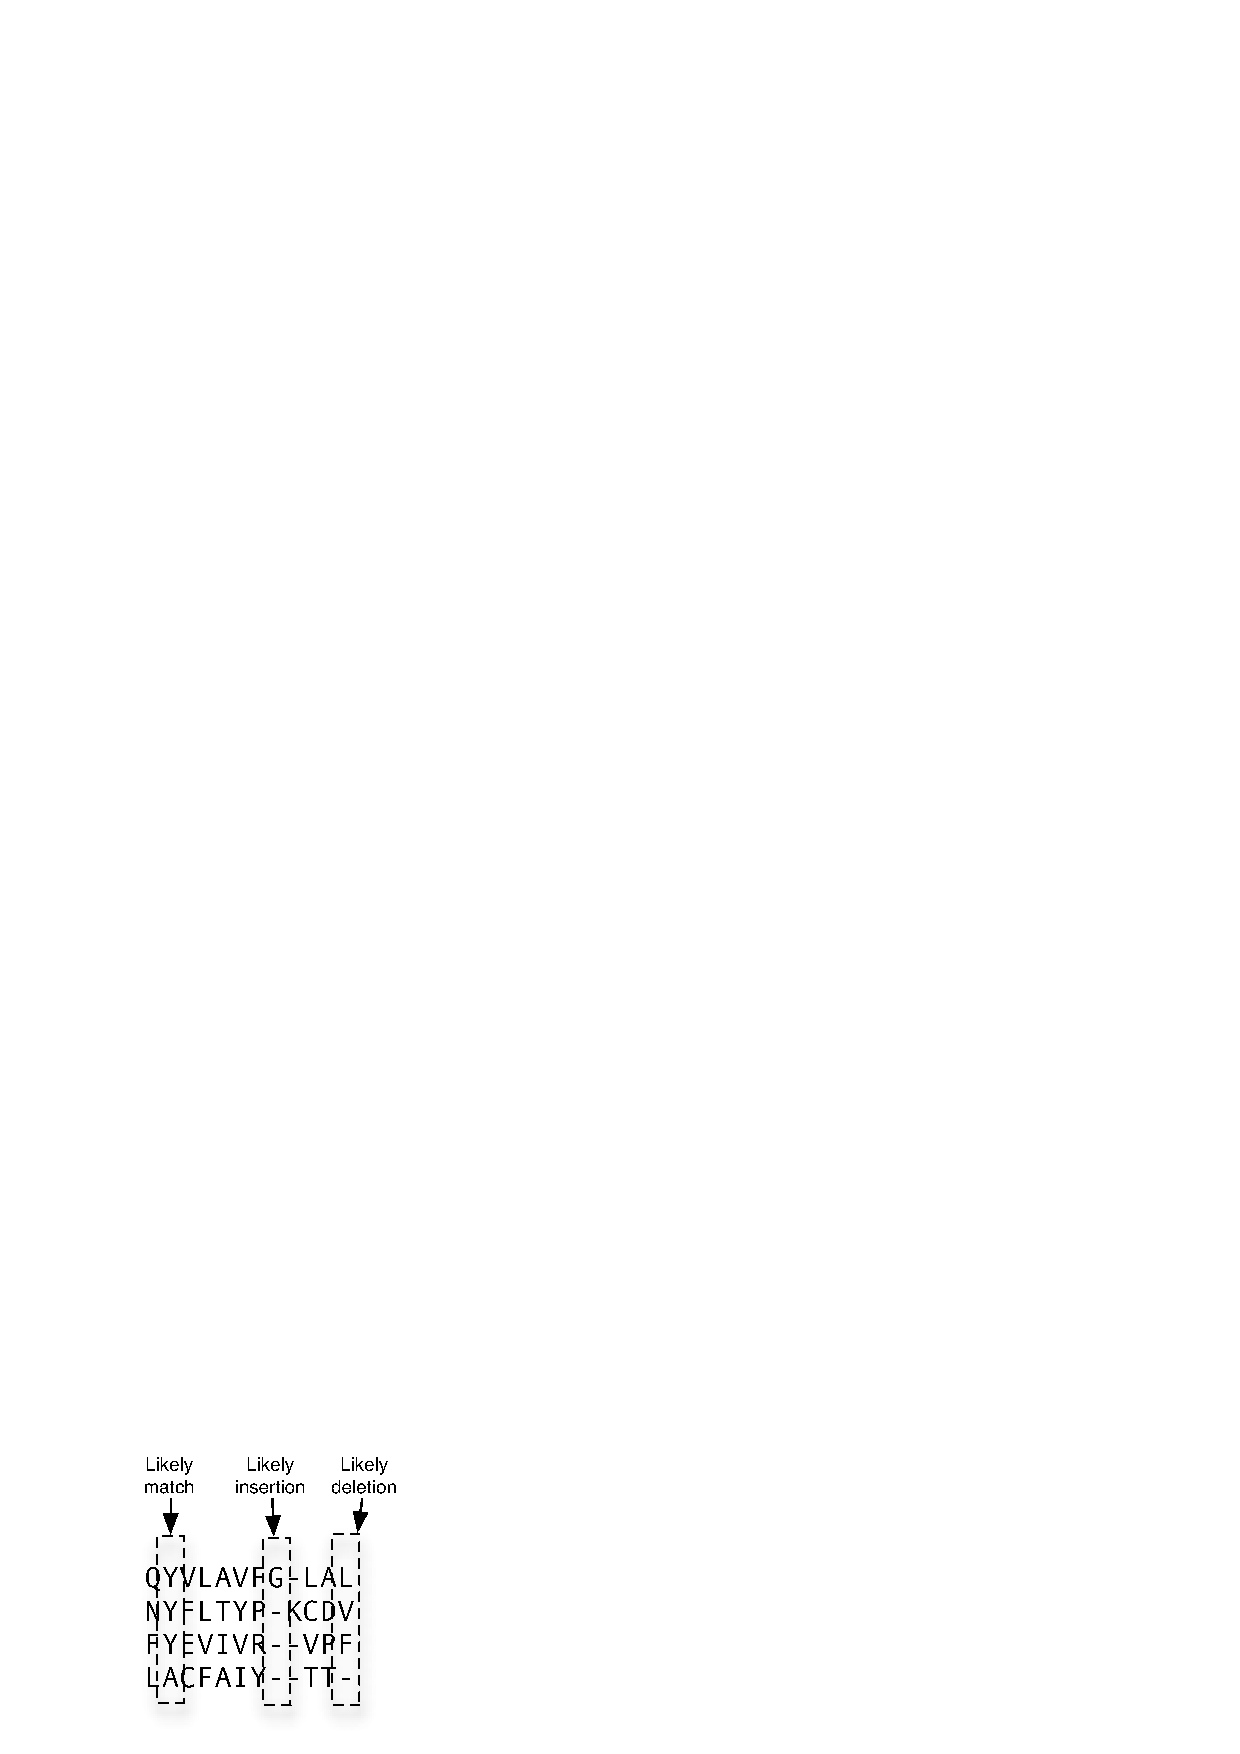
\includegraphics[width=6cm]{alignment.pdf}} 
\caption{Protein sequences are put into alignment based on structural or 
sequence similarities. Each column of the alignment corresponds to a node of 
the hidden Markov model; columns with many gaps will induce highly probable 
insertion states in the HMM, while columns with fewer gaps will induce 
more-probable deletion and match states. Columns with strong consensus towards 
a particular residue will induce match states with high emission probability 
for that residue.}\label{alignment} \end{figure}

The resulting match states, as well as \textit{insertion} states that allow 
additional residues to appear in a protein sequence, and \textit{deletion} 
states that allow match states to be skipped, form a directed graph, the hidden 
Markov model (Figure~\ref{plan7}). Each match or insertion state has an 
associated table of emission probabilities, which correspond to the probability 
of seeing each specific amino acid letter at a given position. Each edge in the 
graph has a weight which is the probability of the associated state transition. 
Triplets of insertion, deletion, and match states are grouped into ``nodes,'' 
which correspond to columns of the original alignment. What looks like an 
intimidating geometry is thus completely explained by the fact that we have 
insertions, deletions, and substitutions due to evolution.

\begin{figure} \centerline{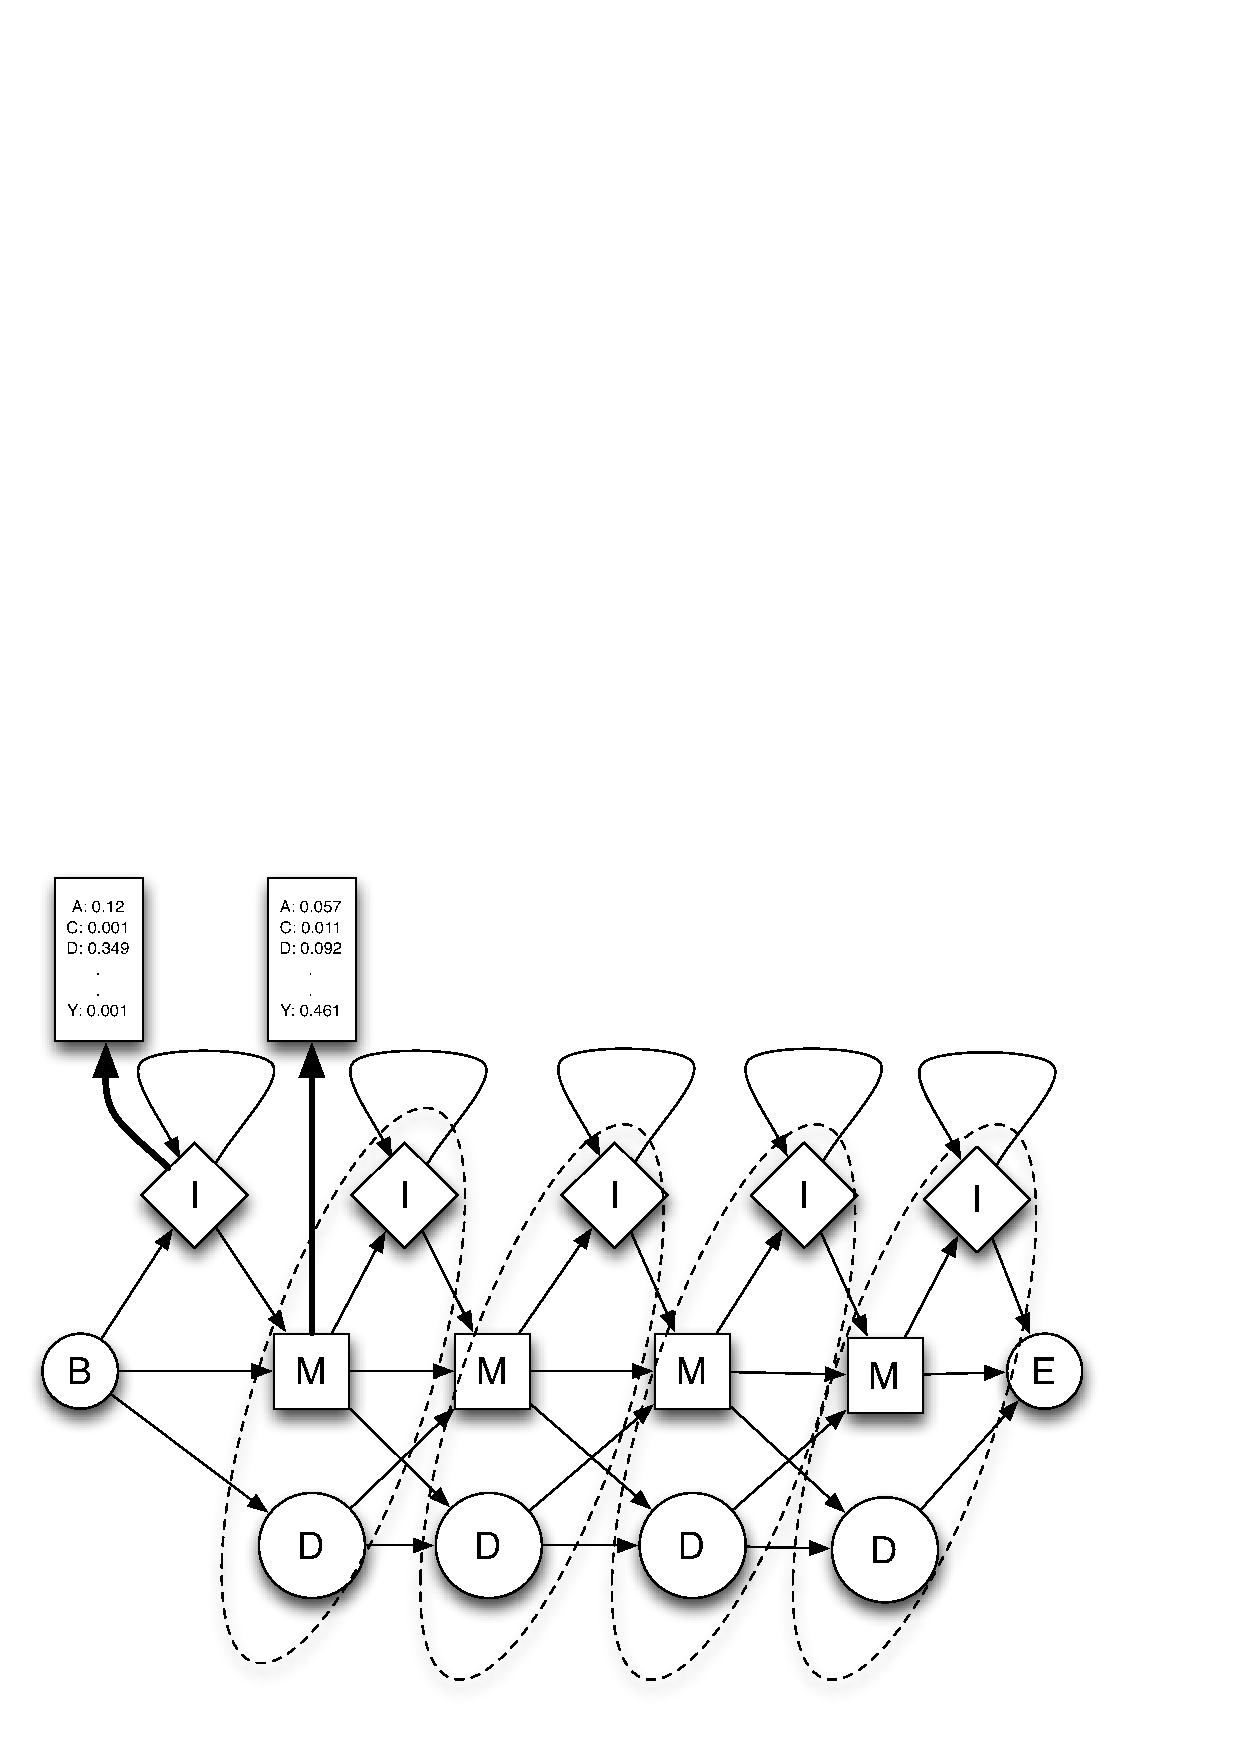
\includegraphics[width=8cm]{Plan7.pdf}} \caption{The 
directed graph representing the states of a traditional HMMER ``Plan7'' hidden 
Markov model. Only 7 of the possible 9 state transitions are allowed, which 
simplifies the dynamic programming. Insertion states represent mutations that 
insert an amino acid, deletion states represent mutations that lose an amino 
acid, and match states represent either conserved amino acids (those with no 
changes) or mutations that substitute one amino acid for another. Each match or 
insertion state has an associated table of emission probabilities (here 
illustrated only for the first two states). Triplets of insertion, deletion, 
and match states are grouped into ``nodes,'' represented here with dashed 
ovals; each node corresponds to a column in the original alignment used to 
train the HMM.}\label{plan7} \end{figure}

If a biologist has trained a hidden Markov model on a group of related 
proteins, she may next use HMMER to determine the likelihood that a new 
protein, whose sequence is known but structure and function are not, shares 
structure and evolutionary history with the proteins that comprise the hidden 
Markov model. HMMER attempts to compute the optimal \textit{parse}, or 
alignment, of a protein sequence onto the directed graph of the hidden Markov 
model. A parse is a mapping of the letters of a query sequence onto the states 
of the model; equivalently, a parse is a \textit{path} through the edges of the 
graph. Since each edge has a weight which is a probability, and each emitting 
state (match or insertion) has a table of emission probabilities, the 
probability of a particular path through the model is simply the product of the 
associated probabilities. This path and its associated probability are computed 
using the Viterbi algorithm~\cite{Viterbi:1967}.


The Viterbi algorithm comprises a set of recurrence 
relations (see Equation \ref{viterbi_eqn}) that seek to maximize the 
probability of an observed sequence (in this case, of amino acid ``letters'') 
being emitted by a particular finite-state automaton (the hidden Markov model). 
To be efficient, the Viterbi 
algorithm relies on dynamic programming, or memoization, and the resulting 
asymptotic complexity is $O(|M|\times|N|)$, when $M$ is the sequence of 
distinct states (nodes in the automaton's graph) and $N$ is the sequence of 
letters in the protein sequence. In our particular problem domain, both $M$ and 
$N$ routinely contain several hundred to a few thousand elements. The types of 
these states and probabilities are provided in Figure~\ref{viterbi_types}.

%% break the viterbi types up and insert into the Plan7 explanation.
%% go over this with NR; I can't make it flow.

\begin{figure}
\lstinputlisting[label=viterbi_types,caption=Viterbi Types]{viterbi_types.hs}
\end{figure}


The textbook Viterbi recurrence relations refer to logs of probabilities, so 
that the terms may be added rather than multiplying raw probabilities. For 
reasons including floating point underflow, the HMMER software (with which we 
maintain file format compatibility) stores all probabilities in a trained HMM 
file as negative natural logs. Thus, the Viterbi recurrence relations are 
simplified from the form in \ref{viterbi_eqn} to that in \ref{viterbi_log_eqn}, 
and because they are \textit{negative} logs, the problem transforms from 
maximization to minimization.


\begin{eqnarray}    
V_{j}^{M}(i) = \log\frac{e_{M_{j}}(x_{i})}{q_{x_{i}}} + max \left\{
\begin{array}{l l}
V_{j-1}^{M}(i - 1) + \log a_{M_{j-1}M_{j}},\\
V_{j-1}^{I}(i - 1) + \log a_{I_{j-1}M_{j}},\\
V_{j-1}^{D}(i - 1) + \log a_{D_{j-1}M_{j}}\\
\end{array} \right.\nonumber\\
V_{j}^{I}(i) = \log\frac{e_{I_{j}}(x_{i})}{q_{x_{i}}} + max \left\{
\begin{array}{l l}
V_{j-1}^{M}(i - 1) + \log a_{M_{j-1}I_{j}},\\
V_{j-1}^{I}(i - 1) + \log a_{I_{j-1}I_{j}},\\
\end{array} \right.\nonumber\\
V_{j}^{D}(i) = max \left\{
\begin{array}{l l}
V_{j-1}^{M}(i - 1) + \log a_{M_{j-1}D_{j}},\\
V_{j-1}^{D}(i - 1) + \log a_{D_{j-1}D_{j}}\\
\end{array} \right.\nonumber\\
\end{eqnarray}\label{viterbi_eqn}

\begin{eqnarray}    
V_{j}^{\prime M}(i) = e^{\prime}_{M_{j}}(x_{i}) + min \left\{
\begin{array}{l l}
V_{j-1}^{\prime M}(i - 1) + a^{\prime}_{M_{j-1}M_{j}},\\
V_{j-1}^{\prime I}(i - 1) + a^{\prime}_{I_{j-1}M_{j}},\\
V_{j-1}^{\prime D}(i - 1) + a^{\prime}_{D_{j-1}M_{j}}\\
\end{array} \right.\nonumber\\
V_{j}^{\prime I}(i) = e^{\prime}_{I_{j}}(x_{i}) + min \left\{
\begin{array}{l l}
V_{j-1}^{\prime M}(i - 1) + a^{\prime}_{M_{j-1}I_{j}},\\
V_{j-1}^{\prime I}(i - 1) + a^{\prime}_{I_{j-1}I_{j}},\\
\end{array} \right.\nonumber\\
V_{j}^{\prime D}(i) = min \left\{
\begin{array}{l l}
V_{j-1}^{\prime M}(i - 1) + a^{\prime}_{M_{j-1}D_{j}},\\
V_{j-1}^{\prime D}(i - 1) + a^{\prime}_{D_{j-1}D_{j}}\\
\end{array} \right.\nonumber\\
\text{where } a^{\prime}_{s} = - \log a_{s} \nonumber \\
\text{and } e^{\prime}_{s,x} = - \log\frac{e_{s,x}}{q_{x}} \nonumber
\end{eqnarray}\label{viterbi_log_eqn}


We implemented the Viterbi algorithm in two distinct ways. We first wrote a 
bottom-up dynamic-programming version, which began with the first node of the 
hidden Markov model and first observation and built up the three-dimensional 
array of possible paths through the model. The array containing the paths 
served as the memoization table. We next wrote a top-down dynamic-programming 
version, which began with the last node of the model and the last observation, 
and applied structural recursion down to the base cases involving the first 
node or first observation (or both). In this second approach, we used the 
\texttt{Data.Memocombinators} library to provide the memoization container 
(again, a three-dimensional array). We determined that the run-time 
performances of both approaches were virtually indistinguishable, and we also 
noted that the top-down version quite faithfully resembled the recurrence 
relations found in a textbook~\cite{durbin} or the HMMER literature~\cite{eddy} 
(see Equation \ref{viterbi_eqn}). We chose to keep the top-down version, which 
later proved to be wise when we had to track down a bug in one of our base 
cases. This bug was observed as a missing state in the alignment our program 
displayed, and we quickly discovered that one of our base cases was missing 
this state: it was returning an empty list as the base of the path, rather than 
a list containing a single node. In this, we were grateful for the resemblance 
between the mathematical description of the algorithm and the top-down 
dynamic-programming approach in Haskell, which resulted in perspicuous code.

\begin{figure*}
\lstinputlisting[label=viterbi,caption=Viterbi]{viterbi_simple.hs}
\end{figure*}


\subsection{MRFy Implementation}

HMMER simply implements the Viterbi algorithm for computing the optimal parse 
of a protein sequence onto a hidden Markov model. Thus, the graphical model of 
a HMMER hidden Markov model is exactly that shown in Figure~\ref{plan7}. In 
contrast, MRFy builds on the approach of SMURF~\cite{smurf} and 
SMURFLite~\cite{smurflite}, our previous work. Like SMURF and SMURFLite, MRFy 
pays attention to longer-range structural interactions than a simple hidden 
Markov model can understand. In particular, these approaches ``nail down'' 
certain subsequences of the model, corresponding to the non-local hydrogen-bond 
interactions between beta strands. Beta strands are regions of protein 
structure that ``stick'' to one another. Because of their pairwise 
interactions, they are highly conserved over the course of evolution. Moreover, 
again because of these pairwise interactions, a change in one amino acid in a 
beta strand may require a change in a corresponding, hydrogen-bonded residue in 
another beta strand if the protein is to remain stable. The architecture of the 
resulting graphical model, derived from the HMMER ``Plan7'' architecture, is 
illustrated in Figure~\ref{mrf}.

These non-local interactions cause what had been a simple hidden Markov model 
to become a Markov random field. SMURF and SMURFLite attempted to compute the 
optimal parse of a protein sequence onto the directed graph representing a 
Markov random field using multidimensional dynamic programming. SMURF's 
computational complexity quickly exploded with complex protein structures, 
while SMURFLite limited its computational complexity by also limiting the 
complexity of protein structure it would understand. The algorithm underlying 
MRFy grew out of an understanding of these limitations.


Rather than attempt to compute exactly the optimal parse, MRFy treats the beta 
strands as ``beads'' which can be slid along a string. In this analogy, the 
string is the sequence of amino acids of the query protein. A given placement 
of these beads corresponds to an assignment of particular amino acid residues 
being hydrogen bonded to other particular amino acid residues, and thus MRFy 
computes a probability based on observed frequencies of residues hydrogen 
bonding in beta strands~\cite{betawrappro}. In between these beta strands, the 
Markov random field is in fact a traditional hidden Markov model, whose optimal 
solution can be easily computed via the Viterbi algorithm. MRFy performs a 
stochastic search to place these beta strands, based on an objective function 
that combines the probability computed by the Viterbi algorithm with that 
computed from the paired, hydrogen-bonded residues in the beta strands. If a 
structure has many beta strands, then it also has many miniature hidden Markov 
models which can be solved via the Viterbi algorithm.


\begin{figure}[h!] 
\centerline{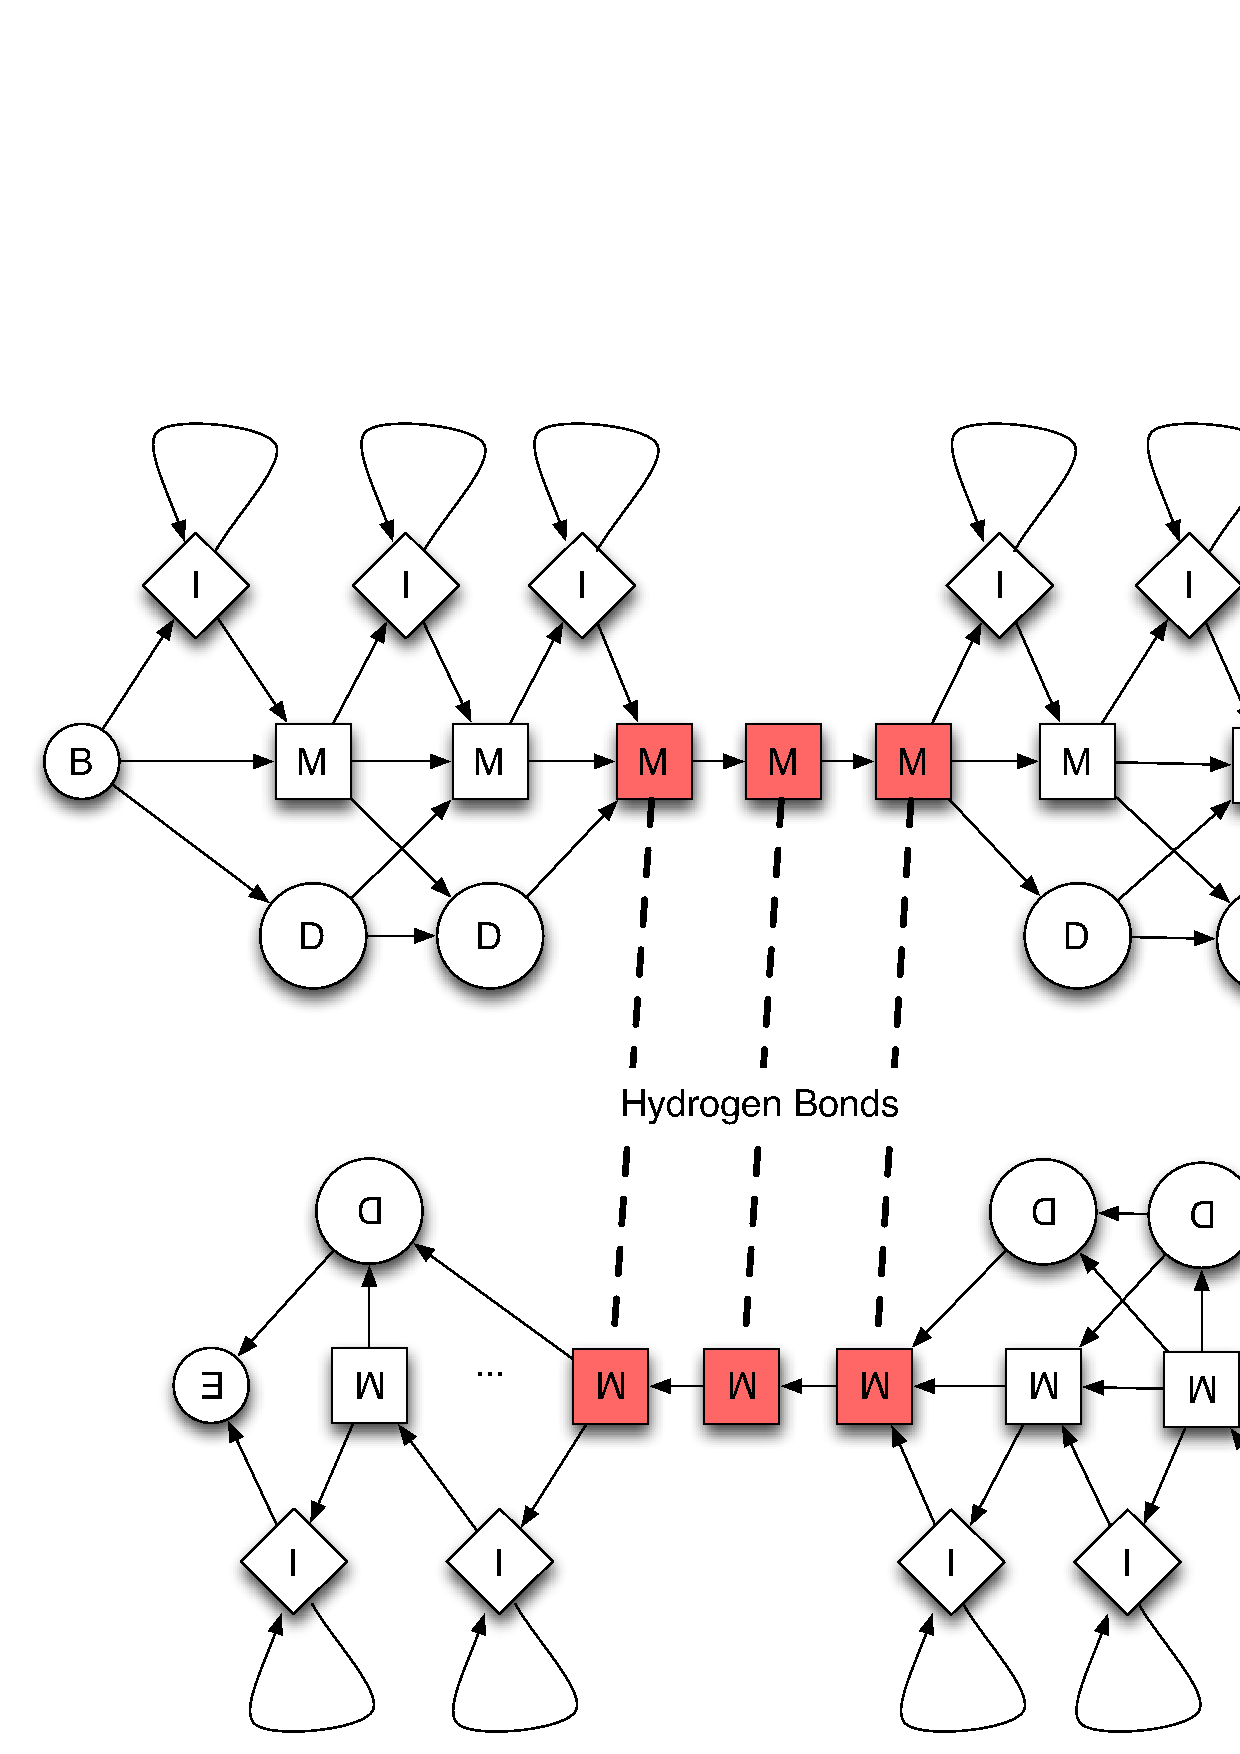
\includegraphics[width=8cm]{mrf_interleave_diagram.pdf}} 
\caption{The directed graph representing the states of a MRFy Markov random 
field finite state automaton. Shaded nodes represent beta-strand positions which have been fixed into match states, 
while the dashed edges represent the long-range dependencies due to hydrogen 
bonding. Note that in between the beta-strand regions are normal HMMs.}\label{mrf} \end{figure}


MRFy contains two distinct algorithms: the classical Viterbi 
dynamic-programming algorithm for hidden Markov models, and a stochastic search 
algorithm for placing beta-strand positions. This stochastic search algorithm 
implements several search heuristics: random-mutation hill climbing, simulated 
annealing, multistart simulated annealing, and a genetic algorithm.


Just as the Viterbi algorithm is one major component of MRFy, stochastic search 
is the other. In designing MRFy, we did not know in advance what sort of 
stochastic search technique would converge the fastest, or give us the best 
alignments with the fastest performance. We decided to implement several 
different search strategies so that we could experiment with all of them. We 
found this to be easy and pleasant thanks to Haskell's support of higher order 
functions.

We wrote a basic search function in only twenty-two lines of code; as one of 
its parameters we provide a \texttt{SearchStrategy} data type, which we use to 
define specific search techniques. We require a \texttt{SearchStrategy} to 
define four functions: \texttt{mutate}, \texttt{accept}, \texttt{terminate}, 
and \texttt{initialize}; we use the Haskell module system to allow sharing of 
some of these functions between different search strategies. For example, both 
\textit{random mutation hill climb} and \textit{simulated annealing} use the 
same initialize and mutate functions, but very different accept functions. In 
all, we implemented four search strategies: \textit{random mutation hill 
climb}, \textit{simulated annealing}, \textit{multistart simulated annealing}, 
and \textit{genetic algorithm}. We found the implementation of the search 
function and search strategies to be pleasant, and the resulting code to be 
simple and elegant. In an imperative language with object orientation like Ruby 
or Python, we likely would have used a class hierarchy to accomplish this. We 
feel that this would have required more code, because object orientation is 
meant for encapsulating data as well as functions on those data; here we only 
wanted to encapsulate functions, as the data did not change.


We note that \texttt{seed} in \texttt{search} comes from a monadic random 
number generator in Main, but we wished for search itself to be pure at this 
level. One advantage is that this allows for testing of the \texttt{search} 
function with no randomness at all: if we pass in a known number as the seed, 
behavior is entirely deterministic.


\begin{figure*}
\lstinputlisting[label=search,caption=Search]{search_simple.hs}
\end{figure*}

In MRFy, the Viterbi function is called several times (once for each 
non-beta-strand region) for each search generation. Furthermore, in a 
population-based search such as \textit{multistart simulated annealing}, the 
scoring function (which itself calls Viterbi) is called many times per 
generation. Beyond traditional profiling, we found parallelization to be an 
obvious way to improve runtime performance. We found this to be trivial thanks 
to the \texttt{Control.Parallel} library. We pass the Viterbi function to a map over all 
non-beta-strand regions of the model and query sequence, and these regions are 
independent of one another. Similarly, we pass the scoring function to a map 
over the population of potential solutions, which are also independent. We 
merely substituted \texttt{parmap rseq} for map. MRFy now efficiently uses all six 
cores on an AMD workstation for a non-population-based simulated annealing 
search, and all forty-eight cores on a compute server for population-based 
searches.


\subsection{Ugly code}


Despite the beauty of some of the code we were able to write, we found several 
instances where the easiest path seemed to be to write ugly code. The first of 
these relates to the otherwise elegant Viterbi function. Our stochastic search 
approach calls the Viterbi function a tremendous number of times, and most of 
the program's runtime is spent in this function. However, the Viterbi algorithm 
retains not just a score (the probability of the sequence given a state path) 
but also the state path itself. We implemented this state path as a list of 
\texttt{Int}, and every step in the recursion conses a new element onto the 
list. However, at each step of the stochastic search, we discard the state 
path; we are searching to optimize score only. We only need the state path at 
the termination of the search, when we wish the program to output an alignment 
of the query sequence to the Markov random field model. We found that 
optimizing the Viterbi function by removing this state path entirely improved 
runtime performance by nearly 50\%. However, we still needed the Viterbi 
function to provide a state path when we called it after search finally 
terminated. Thus, we wondered how to implement the Viterbi function so that a 
state path was optional.

In order to determine if this optimization was even worthwhile, we first wrote 
a quick and dirty approach that is shameful in any language, but easy: we 
duplicated code. We copied \texttt{viterbi} to produce a \texttt{viterbiF} 
which did not retain state path. Next, however, we wondered how to avoid code 
duplication. Clearly, littering the code with conditionals would produce code 
that was ugly as well as less efficient. We knew how we would solve this 
problem in other languages; we would have used macros in Lisp, or 
metaprogramming via \texttt{eval} in Ruby, to produce two versions of the 
function from one prototype. We struggled, however, to solve this problem 
idiomatically in Haskell.

Rather than attempt to use \texttt{TemplateHaskell} to generate two versions of 
the Viterbi function, we wrote a higher-order function type 
\lstinline!type ScorePathCons a = a -> [a] -> [a]! and two functions conforming to that type. 
Then, depending on whether \texttt{viterbi} was called with \texttt{consPath} 
or \texttt{consNoPath} as a parameter, the path would or would not be 
allocated. We found this higher-order function approach to be simple in code 
and in concept, and it imposes negligible run-time overhead as compared to 
having two distinct functions.

\lstinputlisting[label=scorepathcons,caption=ScorePathCons]{scorepathcons.hs}

Another source of ugliness resulted from adding cost-center annotations when we 
wished to profile our code. GHC will happily add cost centers to top-level 
functions, but much of our program relies on sub-functions. We found that 
manually adding \texttt{\{-SCC -\}} annotations to dozens of guard clauses and 
sub-functions harmed the readability of our program, such that we felt 
compelled to remove all such annotations as soon as we could. In our prior 
experience with profiling tools such as kcachegrind, simply compiling with 
debug symbols -- rather than manually annotating many lines of code -- allowed 
the profiling tools to provide us enough information. Without these 
annotations, both call-site and allocation profiles are relatively useless in 
GHC. Perhaps a compile-time flag that would auto-annotate every equation -- 
even if the resulting cost center is simply named with a line number -- would 
make this task easier.

The final source of ugliness in our code came from attempts at debugging 
run-time errors. MRFy relies on a source of input data -- the paired beta 
strands in the Markov random field -- which is represented in an awkward manner 
by the original SMURF program, and which is outside our control. Rather than 
represent beta strands directly, SMURF represents pairings of residues, leaving 
us to infer and reconstruct beta strands. This task was difficult due to 
unclear invariants around overlapping, doubly-paired beta strands (and it would 
have been difficult in any programming language; the difficulty was one of 
representation). However, the debugging tools in GHC caused us some 
difficulties in determining the sources of run-time errors. We used 
\texttt{trace} extensively, but this style of ``\texttt{printf} debugging'' 
littered our code. Being initially unaware of the backtrace feature of the GHC 
profiler, we wrote wrappers around \texttt{Vector.slice} and \texttt{Vector.!} 
which themselves called trace, which at least kept our ``\texttt{printf} 
debugging'' less cluttered. Nonetheless, we struggled with these runtime errors 
due to an awkward representation, and wished for debugging tools such as we 
might find in gdb, which would allow us to examine the stack when a backtrace 
occurs.
 
 
\section{Our previous code base compared}

Our previous computational biology projects include an enhancement to a protein 
structural aligner that previously came from our group, Matt~\cite{matt}. 
Matt's code base contains approximately 12,000 lines of C++ code, and relies on 
data structures such as mutable oct-trees, vectors, and arrays, with 
significant amounts of clever pointer arithmetic. Our enhancement involved 
modifying Matt to incorporate sequence information along with the structural 
aligner. While we initially estimated this would be a three-month project, it 
took most of a year because the mutable data structures were difficult to 
repurpose, and the pointer arithmetic was too clever for its own good: since 
invariants were not clear, nearly every change resulted in new segfaults. One 
enhancement, partial alignments (essentially a cosmetic manipulation of the 
output, but requiring deep information about some of the data structures) was 
deemed infeasible. We believe we could have completed a ground-up rewrite in 
Haskell, with most of the run-time performance, in fewer than nine months.


In general, the failure modes we encounter most in C++ programming are 
segmentation faults, memory errors (due to pointer arithmetic and uninitialized 
memory) and heap exhaustion. In contrast, the failure modes we most commonly 
see in Haskell code are type-check failures, or at worst, runtime errors around 
bounds checking of arrays and vectors. While bounds checking failures have 
proved difficult to debug, they are still less so than C++ memory errors.


Haskell makes it difficult to write code in haste, because Haskell militates 
towards careful type-checking and clearly thought-out function contracts. 
Unlike dynamic languages such as Ruby, and unlike C++, Haskell punishes the 
programmer who attempts to write code quickly with the goal of later making it 
work correctly. We have found MRFy to be easier to enhance and maintain than 
our existing C++ code bases. Despite the learning curve of Haskell, we 
implemented most of MRFy in roughly three months of part-time work.

 
\section{State of the practice}

\subsection{Our group then}
 - Modifying Formatt took nearly a year
 - mutable data structures hard to repurpose
 - one enhancement deemed infeasible
 - C++ failures most commonly segfaults, memory errors, heap exhaustion

\subsection{Our group now}
 - Higher order functions militate towards more flexibility
 - Haskell failures are usually typecheck failures; at worst runtime errors around bounds checking
 - MRFy about 3 months of part-time work

\subsection{Computational biology at large}
 - some good software, like HMMER

\section{What we think about it}

\subsection{Barriers}

- profiling
- debugging
 [ talk about profiling and debugging problems where?]
[ something about quickcheck: how do we know when we have enough QC props? How do we start testing a complex module? ]

\subsection{What you must know to succeed}
- Ecosystem is loaded with tools that look promising but either are no longer maintained or are not ready for prime time (Pads, Backtrace)

\subsection{Evaluation}
- What does the local expert do? Do you have to have one?

- To the FP community: Those who want us to abandon our old tools for debugging imperative code have not provided a clear path to follow (both intellectually, and via software tools).

- No obvious body of knowledge on code improvement.

- The ecosystem contains tools that look promising and work great: Data.Memocombinators, Quickcheck, Parallel Strategies. How to tell what's good? How did we discover what's good?
- Profiler can produce backtraces, but this was hard to discover.

% \appendix
% \section{Appendix Title}
% 
% This is the text of the appendix, if you need one.

\acks

We thank Lenore Cowen, Kathleen Fisher, Benjamin Hescott, Bradford Larsen, and Nathan Ricci.

% We recommend abbrvnat bibliography style.

\bibliographystyle{abbrvnat}

% The bibliography should be embedded for final submission.

\begin{thebibliography}{}
\softraggedright

\bibitem[Smith et~al.(2009)Smith, Jones]{smith02}
P. Q. Smith, and X. Y. Jones. ...reference text...

\end{thebibliography}

\end{document}
